\chapterimage{map.png}
\chapter{Arquitecturas Distribuidas}
\vspace{60px}
\begin{flushright}
\textit{Información obtenida de los siguientes papers \cite{DLT2019}}.
\end{flushright}

\section{Tecnología Ledger distribuido }
La tecnología Ledger distribuido (DLT) ha emergido como una de las tecnologías más disruptivas de la década junto a otras como se puede apreciar en la Figura \ref{fig:tecdisr}. Promete cambiar la manera en que las personas hacen negocios, hacen seguimiento de sus productos y administran su data personal.
\begin{figure}
    \centering
    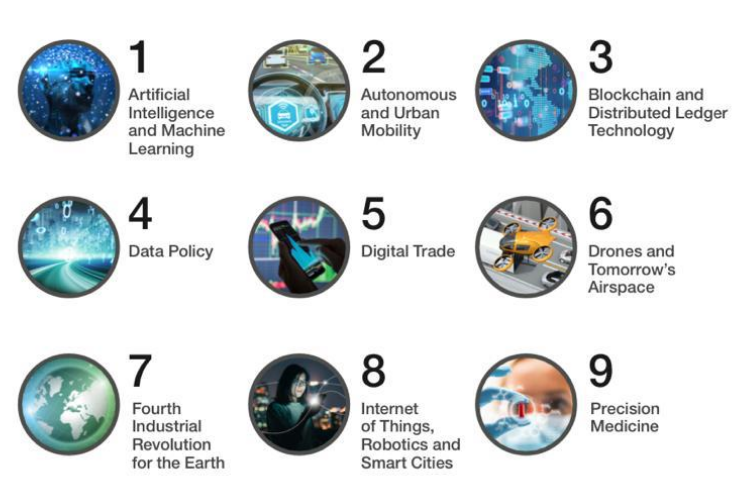
\includegraphics[scale=0.5]{Pictures/tecnologiasdisruptivas.png}
    \caption{Caption}
    \label{fig:tecdisr}
\end{figure}
Las propiedades inherentes que los DTLs proponen a los aplicativos que se monten sobre estos son la \textit{resiliencia},  \textit{integridad}, \textit{anonimato}, \textit{descentralización} y \textit{control autónomo}, las cuales han hecho a muchos adoptar de manera temprana esta tecnología en casi todos los dominios. 
Una forma de ledger distribuido es Blockchain, el cual fue implementado en 2009 para permitir el surgimiento de criptomonedas como Bitcoin. 
Por tanto Blockchain es solo un ejemplo particular donde los datos pueden ser almacenados en un formato específico. Cuando el ledger está distribuido en una red, entonces se le llama ledger distribuido.

Blockchain es una tecnología de ciberseguridad matemática para la identificación rápida y sin duda de modificaciones en datos digitales o dispositivos inteligentes.
\textbf{Blockchain garantiza seguridad sobre redes que no son confiables porque las partes puede realizar transacciones incluso con otros en los que no confían}. 
%
e-stonia define al Blockchain como un polvo de defensa digital que permite dejar la traza de quienes intentan modificar los bloques que componen esta cadena. 
%
Para nosotros los informáticos, una Blockchain es una estructura de datos distribuidas que está replicada y es compartida entre los miembros de una red. Cada bloque en la cadena lleva una lista de transacciones y un hash al bloque previo. La excepción se le permite sólo al primer bloque de la cadena, llamada \textbf{génesis}, que es común a todos los clientes en una red blockchain (claramente no tiene padre). Una blockchain en términos de las ciencias de la computación también puede ser visto como un log cuyos registros son almacenados en bloques con marca de tiempo. 

\begin{figure}
    \centering
    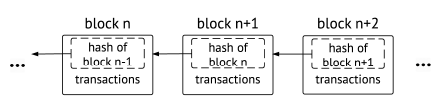
\includegraphics{Pictures/bloques.png}
    \caption{Estructura de datos de blockchain}
    \label{fig:estrdatos}
\end{figure}

%
Por tanto, el ledger (libro mayor) consiste de bloques consecutivos encadenados siguiendo un conjunto estricto de reglas. El ledger es distribuido y almacenado por los nodos P2P de la red donde cada bloque es creado por un intervalo predefinido de una manera descentralizada y gobernada por algoritmos de consenso que garantizan la integridad de los datos. Esto permite además que el ledger distribuido sea sincronizado por los múltiples nodos. Bitcoin introdujo el Proof-of-Work como algoritmo de consenso.


En general, un ledger exhibe multiples propiedades: 

\begin{itemize}
    \item Consenso distribuido respecto del estado del ledger.
    \item Inmutabilidad e irreversibilidad del estado del ledger. 
    \item Persistencia de los datos (transacciones).
    \item Trazabilidad de los datos.
    \item Control de datos distribuidos.
    \item Transparencia y responsabilidad (accountability).
\end{itemize}



\subsection{¿Cómo funciona blockchain?}\label{secc:BC}
Un conjunto de nodos operan en la misma blockchain vía la copia que cada uno tiene. Por simplicidad asumiremos que un usuario realiza transacciones en la red vía su propio nodo (un nodo puede generalmente actuar como un punto de entrada para diferentes usuarios de la blockchain). Estos nodos forman una red P2P donde:


\begin{itemize}
    \item Usuarios interactúan con la blockchain vía llaves privadas/públicas. Ellos usan su clave privada para firmar sus transacciones, y estas serán encontrables en la red usando la clave pública. El uso de criptografía asimétrica permite \textit{autenticación}, \textit{integridad} y \textit{no repudiación} en la red. Toda transacción firmada es reenviada por un nodo de usuario a todos los otros con distancia ``un salto''. 
    \item Los vecinos se aseguran que la transacción que llega sea válida; sino la descartan. Eventualmente esta transacción es esparcida por la red. 
     \item Las transacciones que han sido recolectadas y validadas por la red usando el proceso anterior durante un intervalo de tiempo acordado, son ordenadas y empaquetadas en un bloque candidato con su respectiva marca de tiempo. 
    \item Los nodos verifican que el bloque sugerido contiene transacciones válidas y referencias mediante hash del bloque anterior correcto en su cadena. Si ese es el caso, entonces, el bloque se adiciona a la cadena, y la transacción es abierta al mundo. Sino, el bloque propuesto es descartado. 
\end{itemize}


%\subsection{¿Cómo se alcanza consenso en la red?}

%\subsection{¿Cómo se transfieren activos digitales en una red blockchain?}
\subsection{¿Cómo funcionan los contratos inteligentes?}\label{secc:CI}

Nick Szabo introdujo el concepto en 1994 definiéndolo como un protocolo de transacción computarizada que ejecuta los términos de un contrato. El objetivo era trasladar todas las condiciones contractuales a código, embebiéndolo en propiedades (del software o hardware) que puede ser forzado a cumplir sin tener que pasar por intermediarios confiables. 

En blockchain, los contratos inteligentes son scripts almacenados en la blockchain. Dado que residen en la cadena, ellos tienen dirección única. Al asociarle una transacción, estos se generan de manera automática. Entonces, ejecutan independientemente lo que deban hacer en cada nodo de la red que corresponda. 

\begin{tcolorbox}[colback=gray!5!white,colframe=orange!60!gray,title=PREGUNTA 1]
Considere que Pedro, Juan y Diego participan en una red blockchain donde los activos digitales X e Y son transados. Juan despliega un contrato inteligente en la red que define: (a) una función de `` depósito '' que le permite depositar unidades de X en el contrato, (b) una función de `` intercambio '' que devuelve 1 unidad de X (de los depósitos propios del contrato) por cada 5 unidades de Y que recibe, y (c) una función de `` retiro '' que le permite a Juan retirar todos los activos que posee el contrato.
%
Si consideramos que las funciones `` depositar '' y `` retirar '' están escritas para que solo Juan (a través de su clave) pueda llamarlas, porque esto es lo que decidió Juan.


Juan envía una transacción a la dirección de ese contrato inteligente, llamando a su función de `` depósito '' y moviendo 3 unidades de X al contrato. Esta transacción se registra en la cadena de bloques.
Pedro, que posee 12 unidades de Y, luego envía una transacción que mueve 10 unidades de Y a la función de `` intercambio '' del contrato, y recupera 2 unidades de X. Esta transacción también se registra en la cadena de bloques. Juan luego envía una transacción firmada a la función de `` retiro '' del contrato. El contrato verifica la firma para asegurarse de que el retiro del contrato sea iniciado por el propietario del contrato y transfiere todos sus depósitos (1 unidad de X y 10 unidades de Y) a Bob. Considere lo siguiente:
\begin{enumerate}
    \item El contrato tiene su propio estado y puede tomar la custodia de los activos en la cadena de bloques. Decimos que un contrato tiene su propia cuenta en la cadena de bloques, y la cadena de bloques admite un modelo basado en la cuenta. En el ejemplo anterior, puede contener los activos X e Y. (Si volvemos para el modelo de base de datos compartida, un contrato es un `` usuario ''/entidad  que puede poseer, eliminar y crear filas.) 
    \item El contrato nos permite expresar la lógica comercial en código; `` intercambiará 1 unidad de X por cada 5 unidades de Y recibidas ''.
\end{enumerate}


\end{tcolorbox}


%%%%%%%%%%%%%%%%%%%%%%%%%%%
\subsection{Proveedores de Blockchain}
El ``ledger de Bitcoin'' evolucionó, y un nuevo tipo de ledger emergió entregando mayores facilidades para el despliegue y ejecución de programas computacionales, conocidos como contratos inteligentes. Estos contratos permiten la creación de aplicaciones descentralizadas (DApps) donde programas autónomos operan sin necesariamente confiar en alguna entidad del sistema. Que los contratos sean parte del ledger hacen a su vez a los contratos inteligentes así como a sus ejecuciones inmutables e irreversibles además de habilitantes de sistemas basados en workflows. 
Claramente esto ha entusiasmado a muchas compañías quienes han propuesto múltiples plataformas, las cuales usualmente pueden ser categorizadas como públicas, privadas, mixtas, de propósito general y específicas. La siguiente es una lista no exhaustiva:
\begin{itemize}
    \item KSI Blockchain (e-stonia)
    \item Bitcoin 
    \item Ethereum 
    \item Hyperledger Fabric 
    \item Hyperledger Sawtooth
    \item Hyperledger Burrow 
    \item EOS 
    \item Multichain 
    \item R3 Corda 
    \item Cardano 
    \item IOTA 
    \item Walton-Chain 
  
\end{itemize}
\begin{remark}
\textbf{Es importante notar que existen proveedores de otros Ledgers distribuidos, donde no necesariamente los bloques apuntan a su predecesor, tales como Neuro-Ledger}.
\end{remark}

Criterios de evaluación para comparar proveedores o alternativas:
\begin{itemize}
    \item Público o privado. 
    \item Escalabilidad: cuanta data un sistema puede procesar en cierta unidad de tiempo
    \begin{itemize}
        \item tamaño del bloque: indica el tamaño máximo de un bloque en el sistema DLT.
        \item tiempo de creación del bloque: especifica el tiempo promedio de la creación del bloque para un sistema particular. 
    \end{itemize}
    \item Costo incurrido por transacción a procesar o data a almacenar en el ledger. El costo en el dominio de Blockchain es referido como la comisión de la transacción.
    \item Consumo de energía: cuanta energía eléctrica es utilizada durante el proceso de creación y minado de bloques. 
    \item Consenso: algoritmo que es usado para alcanzar consenso distribuido. Esto está correlacionado con el tiempo de creación de bloques como del consumo de energía.  
    \item Privacidad.
    \item Identidad y auditabilidad
    \item adecuabilidad para diferentes tipos de datos, tamaños, volumen, entre otros.
    \item robustez y resiliencia frente a ataques y errores nunca antes vistos.
    \item Nivel de confianza: analiza el nivel de confianza de un sistema en término de su adopción.
    \item Gobernanza: mecanismo de gobierno abierto y público que aumente el nivel de confianza en el sistema.
    Extendible: si sobre este es posible agregar nuevas funcionalidades o rectificar errores. 
    \item sostenibilidad. 
\end{itemize}

\section{X-road}
X-Road es un sistema para permitir una comunicación segura entre organizaciones, de manera \textit{descentralizada} sin intermediarios. Se dice que es una plataforma de interoperabilidad entre organizaciones pues estandariza el protocolo de comunicación entre ellos. Utiliza protocolos seguros de comunicación, que no generen cuellos de botella ni  puntos únicos de falla. Toda comunicación entre las organizaciones se comunica mediante llamadas a servicio (REST o SOAP), donde una vez conectada una organización a la infraestructura X-road puede actuar como cliente y/o proveedor de servicio. \textbf{Es capaz de conectarse con servicios fronterizos de organizaciones que usen una instancia diferente de X-road.} Todo mensaje procesado por X-road puede ser usado como evidencia digital dado que llevan sellos digitales (SSCD).


\begin{figure}[h!]
    \centering
    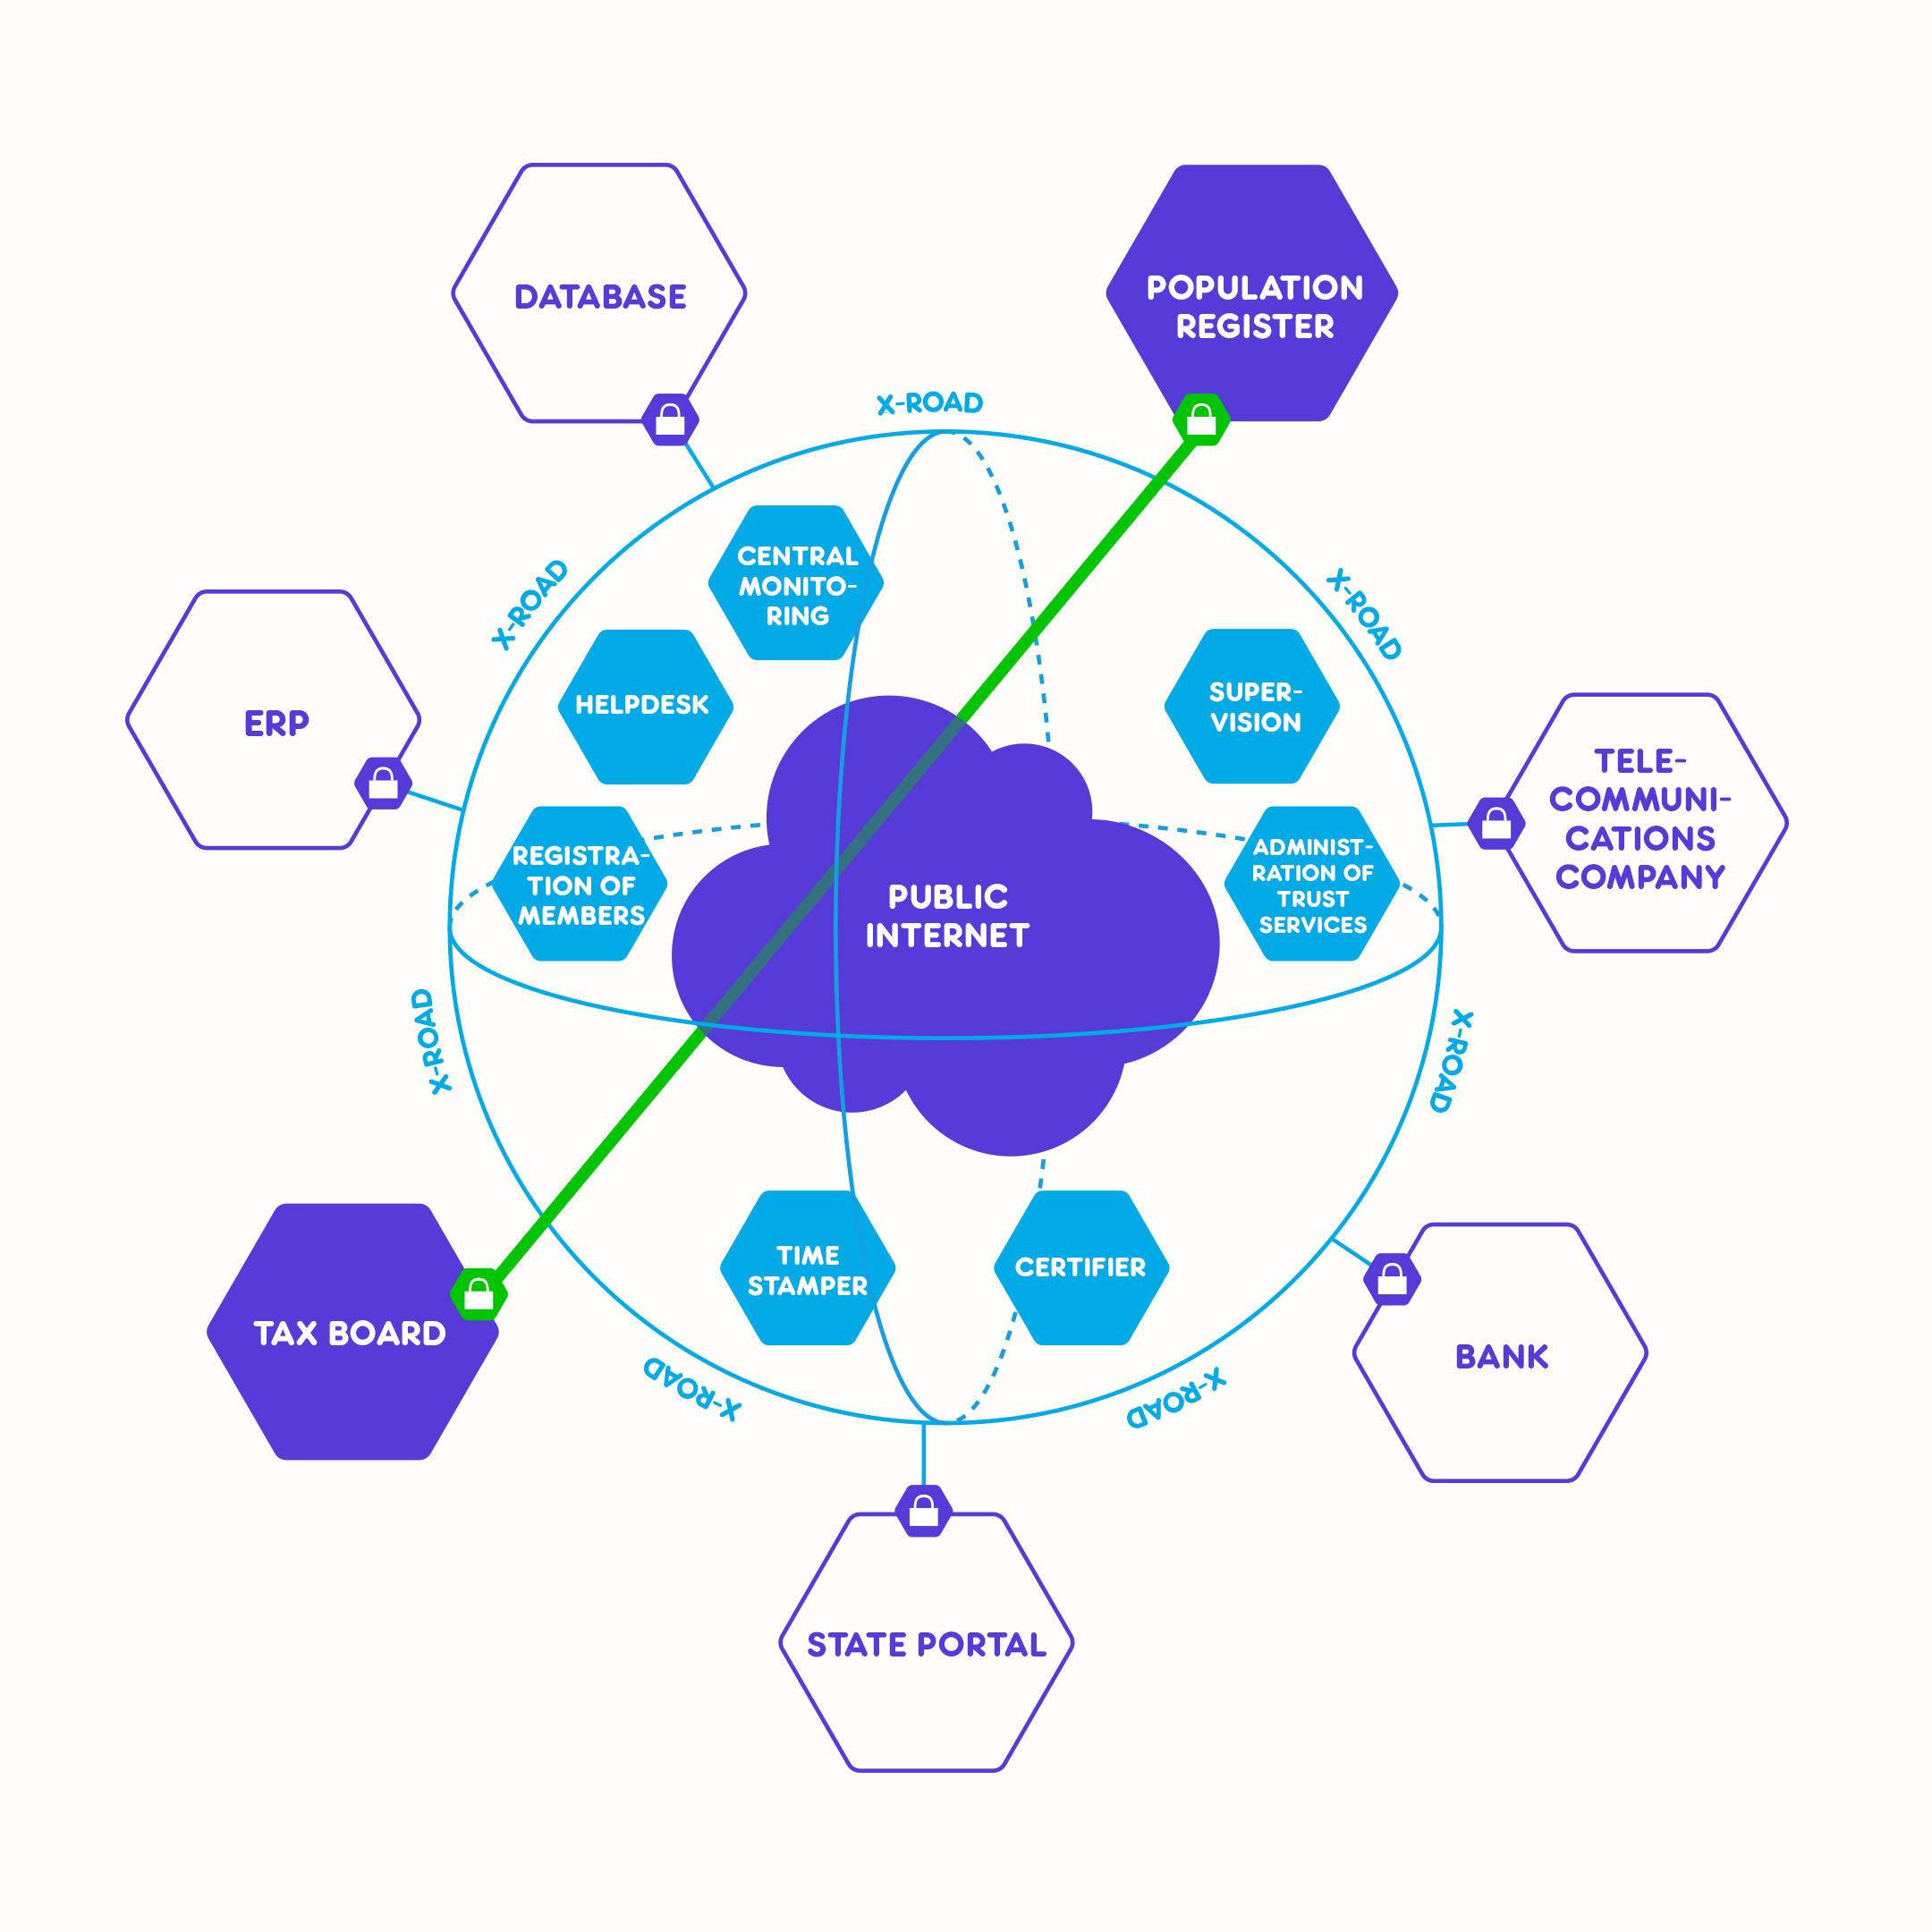
\includegraphics[scale=0.20]{Pictures/X-Road_overview.png}
    \caption{Vista global de X-road. }
    \label{fig:X-road}
\end{figure}

En la Figura \ref{fig:DC}  se ven los componentes de X-road. El \textbf{servidor central} administra la base de datos de los miembros de X-road y los \textbf{servidores de seguridad}. El servidor central contiene la base de datos de miembros y la política de seguridad (accesible desde los servidores de seguridad vía HTTP) compuesta de \textbf{autoridades de certificación}, \textbf{autoridades de marca de tiempo} y otros parámetros. Otros servicios que provee son agregar o remover clientes servidores de seguridad (las que son invocadas desde la interfaz usuaria de los servidores de seguridad). 
\begin{figure}[h!]
    \centering
    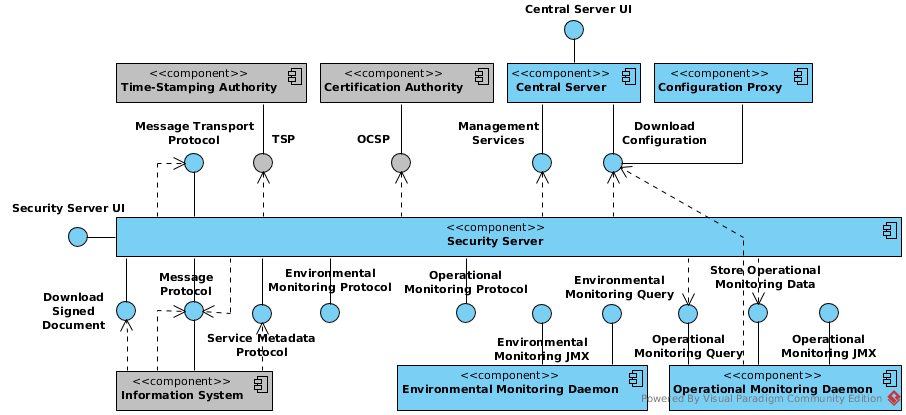
\includegraphics[scale=0.6]{Pictures/arc-g_logical_structure_of_x_road.png}
    \caption{Diagrama de componentes. Componentes  en plomo no son provistos por X-road.}
    \label{fig:DC}
\end{figure}

El \textbf{servidor de seguridad} media las llamadas a servicios y respuestas encapsulando los aspectos de seguridad de la infraestructura X-road administrando llaves para firmar y autenticar, enviando mensajes sobre el canal seguro, creando el valor de prueba para mensajes con firma digital, marca de tiempo y logs. Ofrece una API mediante SOAP/REST. 
Un \textbf{servidor de seguridad}  puede albergar más de una organización. 

El \textbf{sistema de información} usa y provee servicios mediante X-road. La \textbf{autoridad de certificación} (CA) emite certificados a los servidores de seguridad (certificados de autenticación) y a las organizaciones miembros de X-Road (certificados de firma). Todos los certificados se almacenan en los servidores de seguridad. La CA debe poder procesar las solicitudes de firma de certificados de acuerdo con PKCS10.


\begin{figure}[h!]
    \centering
    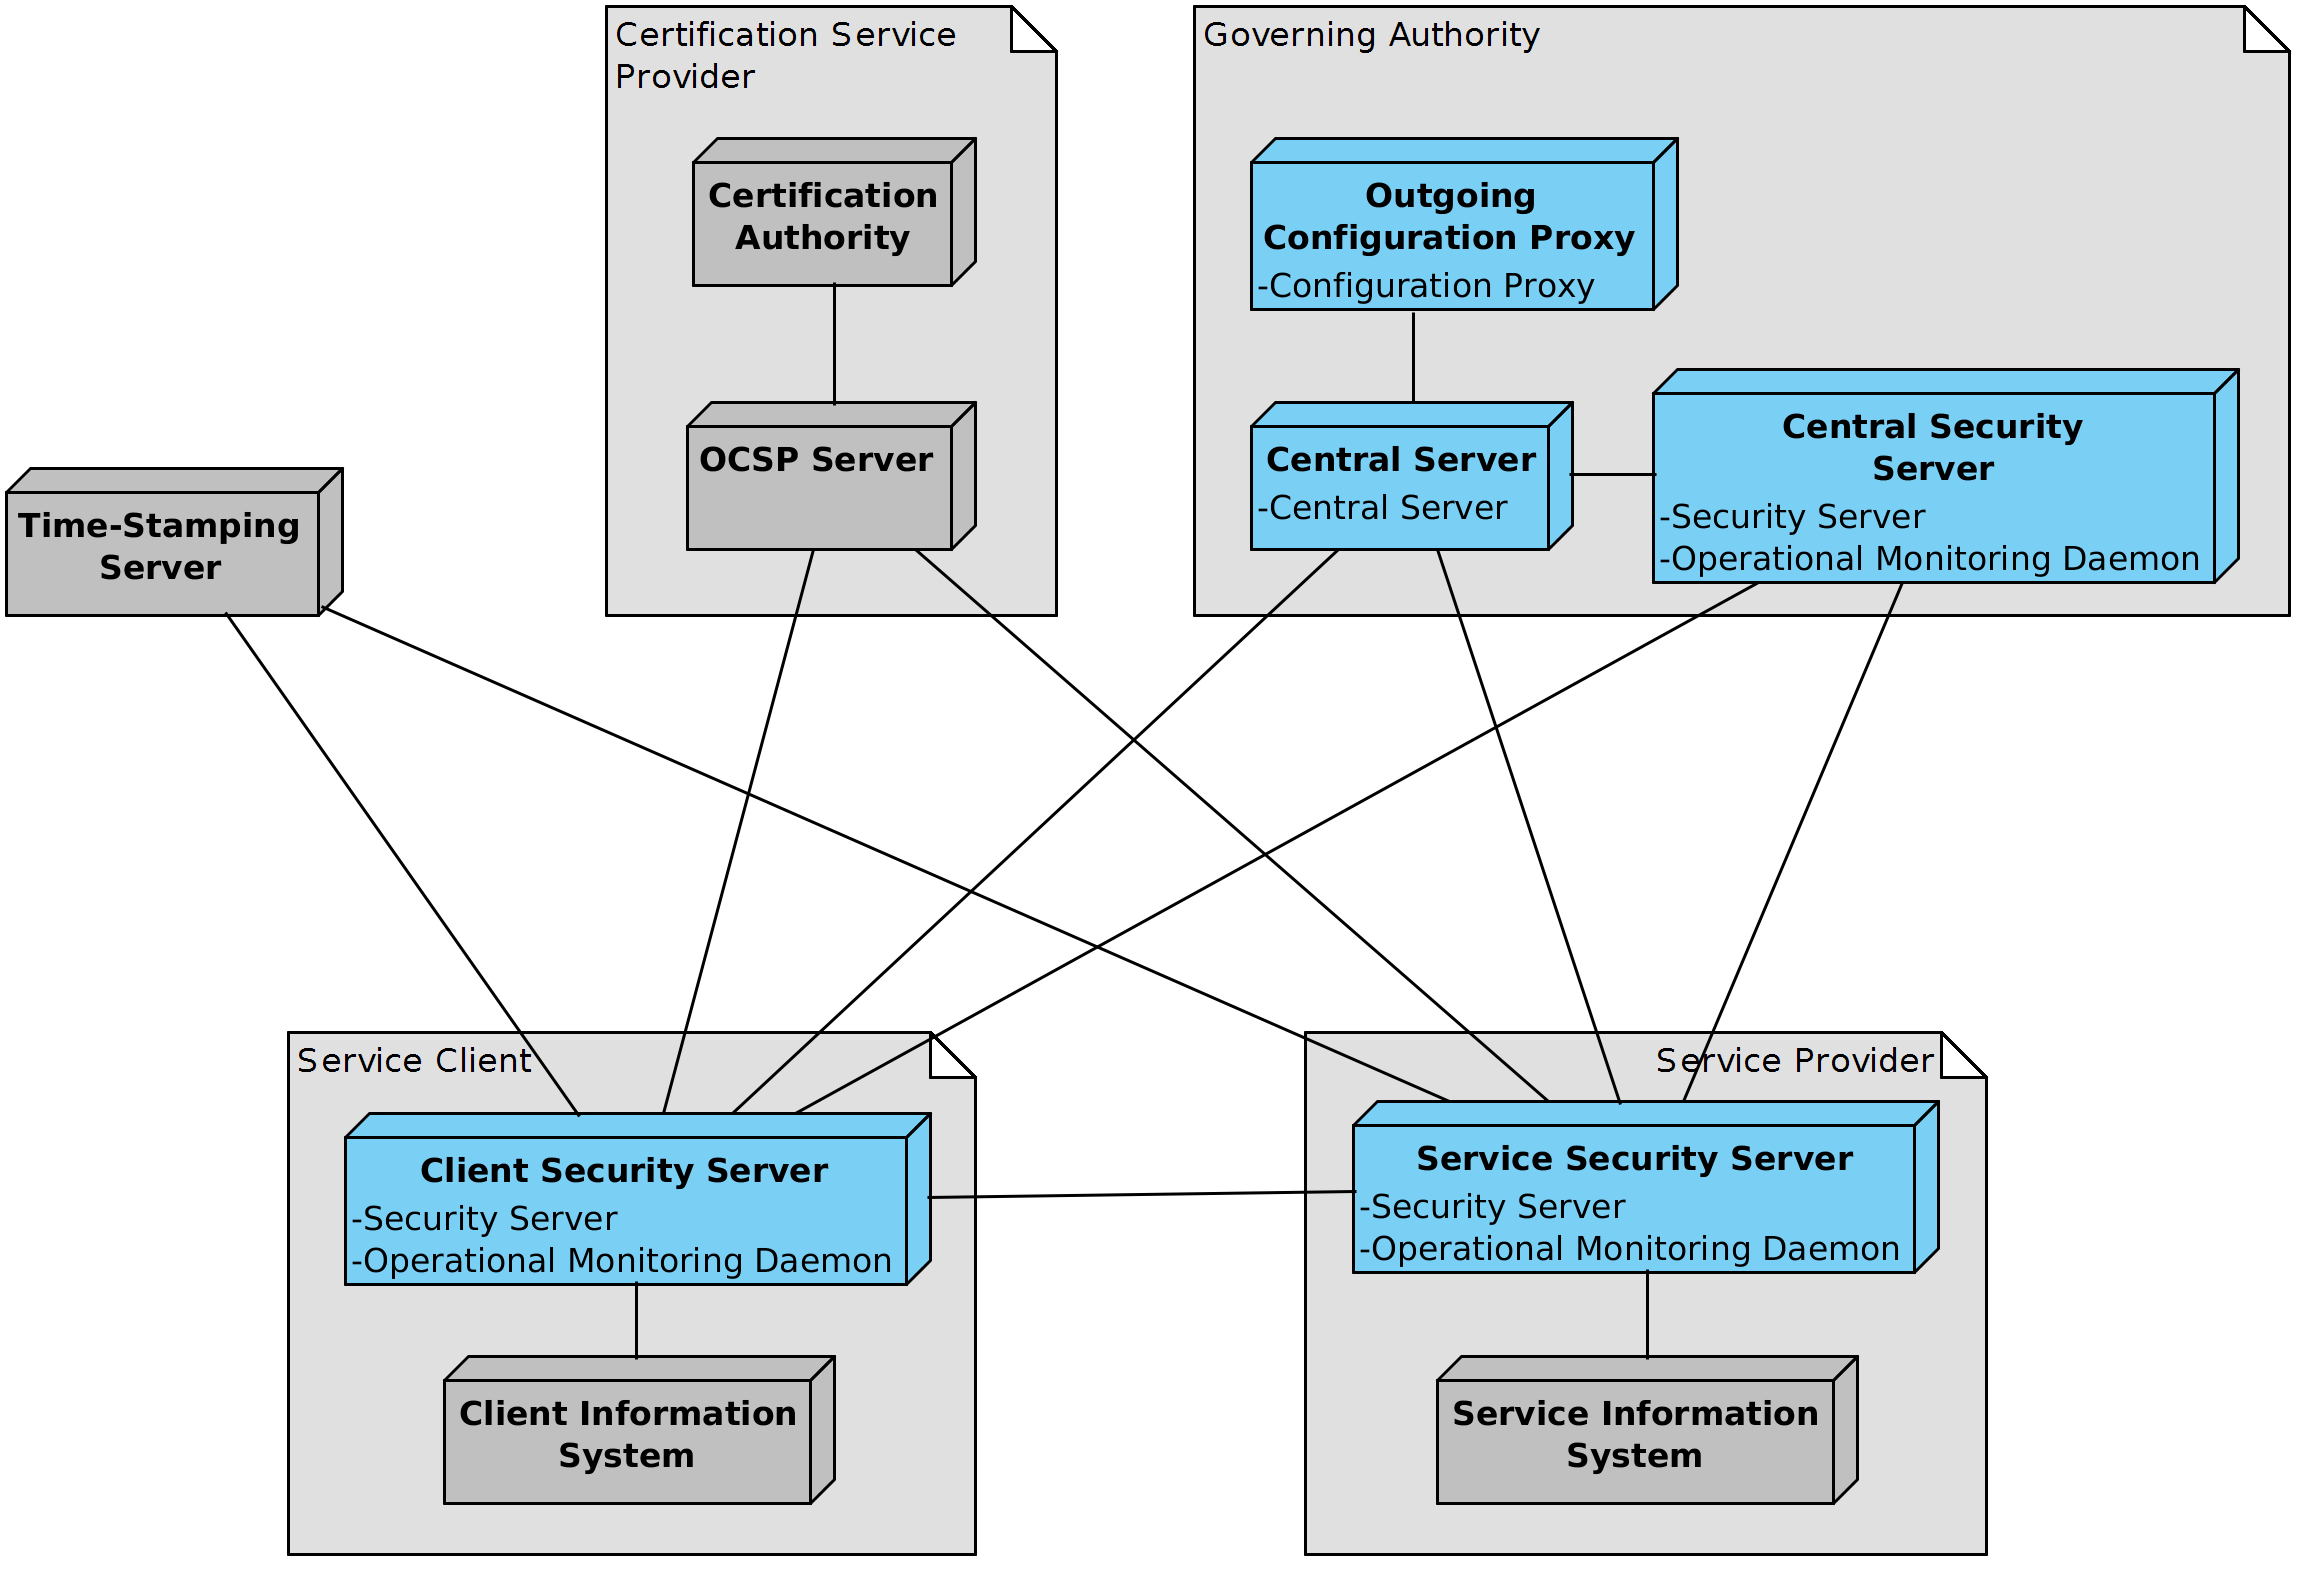
\includegraphics[scale=0.7]{Pictures/arc-g_deployment_view_of_x_road.png}
    \caption{Diagrama de despliegue}
    \label{fig:DD}
\end{figure}

La Figura \ref{fig:DD} muestra la vista de implementación de una instancia básica de X-Road. En la práctica, todos los componentes pueden usar redundancia para mejorar la \textit{disponibilidad} y el \textit{rendimiento}. 

El diagrama también muestra qué componentes están instalados y alojados por una organización determinada. La autoridad de gobierno instala y mantiene el \textbf{servidor central} y el \textbf{servidor de seguridad central}. El \textbf{proxy de configuración} es un componente opcional que generalmente se usa para distribuir la configuración a instancias federadas de X-Road. Las organizaciones de clientes y proveedores de servicios alojan su sistema de información y servidor de seguridad que conecta el sistema de información a X-Road.


\section{Tarea}
\begin{itemize}
    \item Mediante Blackboard la entrega debe ser el domingo 9 de agosto - 2359. Descuentos por atrasos injustificados: desde 1 segundo a 23 horas 59 minutos 59 segundos: 1 punto. (recuerde siempre conversar con su profesor).
    \item Es obligatorio el uso de UML y del software starUML. Debe entregar todos los modelos en un proyecto starUML (extensión mdj). Descuento máximo relativo respecto de proyectos con elementos repetidos o sin conexión entre diagramas.
    \item Los grupos de trabajo son máximo 5. 
    \item Debe entregar informe de Tarea 1 cuidando aspectos formales  y básicos de un documento tales como índice general y de figuras. (descuento máximo 1 punto de escala de 1 a 7)
    \item Cada diagrama debe tener supuestos, raciocinio y explicación de cada componente, conexión u otro que aparezca en el diagrama. Descuento máximo relativo a este tema: 0,5 punto por diagrama.
    \item Cada diagrama debe tener una discusión respecto de los atributos de calidad. Descuento máximo relativo a este tema: 0,5.
    \item Debe tener una bitácora al final de trabajo del aporte que hizo cada integrante (indicando fecha y hora). 
\end{itemize}


\subsection*{Pregunta 1}

\begin{flushright}
   Entregar en .mdj \textit{(4 puntos)}
\end{flushright}
%\vspace{20px}

\begin{remark}
TODOS LOS DIAGRAMAS DEBEN SER UTILIZADOS EN STARUML. SI DEBE HACER UN DIAGRAMA DE SECUENCIA (DE INSTANCIAS DE COMPONENTES), PRIMERO DEBE CREA UN DIAGRAMA DE COMPONENTES Y ARRASTRAR EL COMPONENTE HACIA EL NUEVO DIAGRAMA. LOS COMPONENTES DEBEN ESTAR INTERRELACIONADOS ENTRE SI. 
\end{remark}
\begin{tcolorbox}[colback=gray!5!white,colframe=red!60!gray,title=SOLO A PARTIR DE LA DESCRIPCION ENTREGADA ACÁ]
\begin{enumerate}
    \item Realizar un diagrama de secuencia de la sección \ref{secc:BC} cómo funciona Blockchain. 
     \item Realizar un \textbf{diagrama de colaboración} (no secuencia) de la sección \ref{secc:CI} cómo funciona CONTRATOS INTELIGENTES. (recuadro naranjo). 
\end{enumerate}

\end{tcolorbox}


\begin{figure}
    \centering
    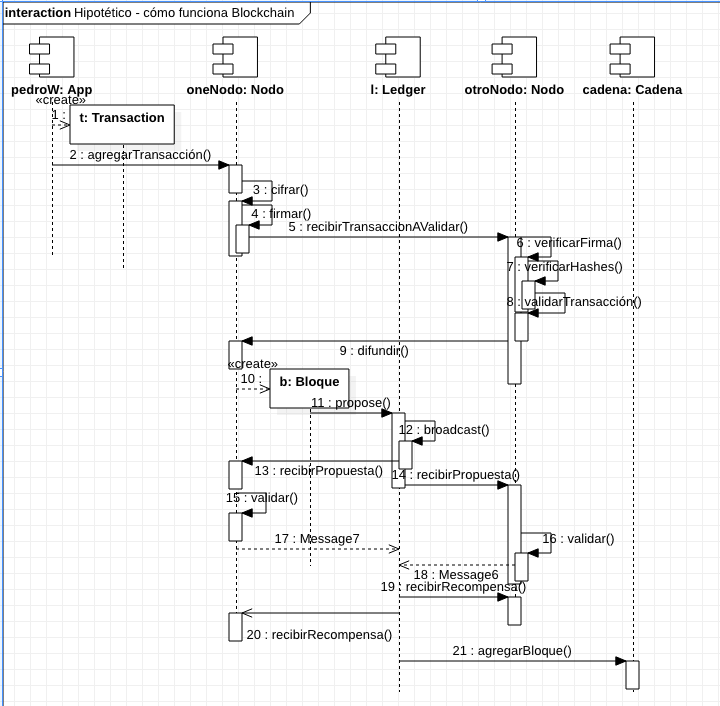
\includegraphics[width=\textwidth]{Pictures/blockchain.png}
    \caption{Diagrama de secuencia del Caso hipotético y simplificado de cómo funciona Blockchain (Pregunta 1.1)}
    \label{fig:p1a}
\end{figure}

\begin{figure}
    \centering
    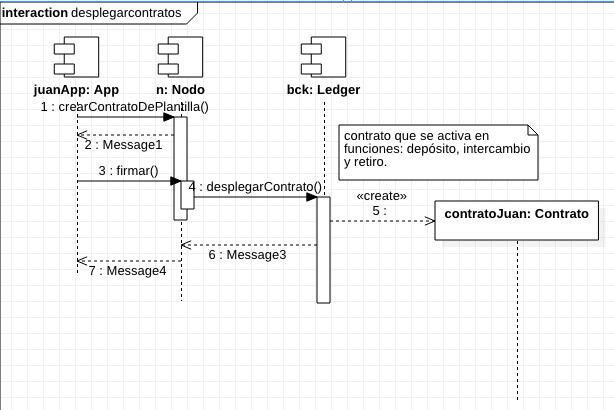
\includegraphics[width=\textwidth]{Pictures/sc.png}
    \caption{Diagrama de secuencia del Caso hipotético y simplificado de crear contrato (parte 1 Pregunta 1.2)}
    \label{fig:sc}
\end{figure}


\begin{figure}
    \centering
    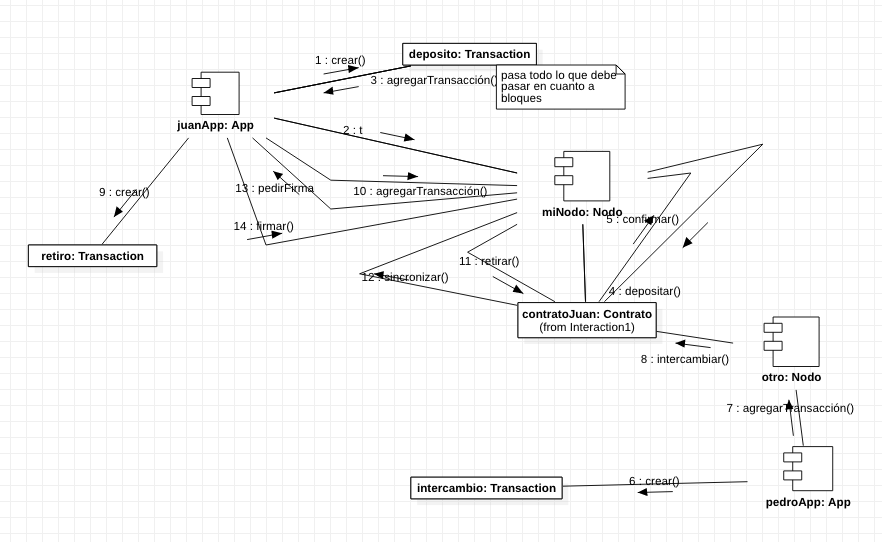
\includegraphics[width=\textwidth]{Pictures/ejecutarcontrato.png}
    \caption{Diagrama de colaboración del Caso hipotético y simplificado de cómo funcionan los contratos (parte s Pregunta 1.2)}
    \label{fig:sc}
\end{figure}

\newpage
\subsection*{Pregunta 2}

\begin{flushright}
    Entregar en .mdj
    \textit{(2 puntos)}
\end{flushright}
%\vspace{20px}

Para el caso del servidor de seguridad de X-road, utilizando la documentación en \url{https://bitbucket.niis.org/projects/X-ROAD/repos/x-road/browse/doc/Architecture/arc-ss_x-road_security_server_architecture.md} (Si tiene problemas con el inglés, utilice chrome y pídale traducir la página) realizar el diagrama de secuencia de lo que se indica en el proceso de la Figura \ref{fig:SSDP}.  

\begin{figure}[h!]
    \centering
    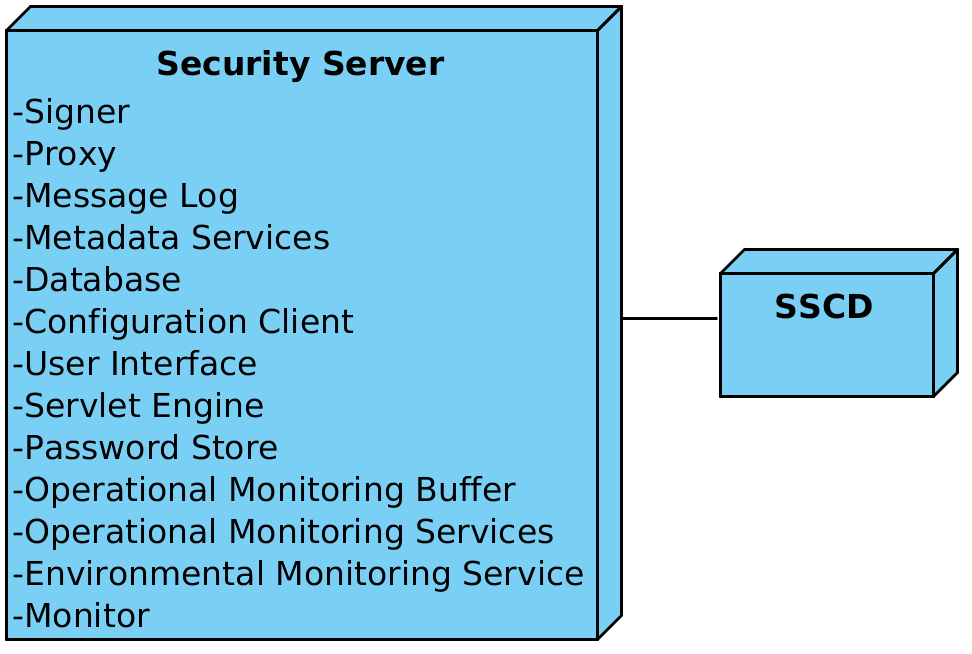
\includegraphics[scale=0.5]{Pictures/arc-ss_simple_security_server_deployment.png}
    \caption{Diagrama de Despliegue del componente \textbf{servidor de seguridad}}
    \label{fig:SSDD}
\end{figure}
\begin{figure}[h!]
    \centering
    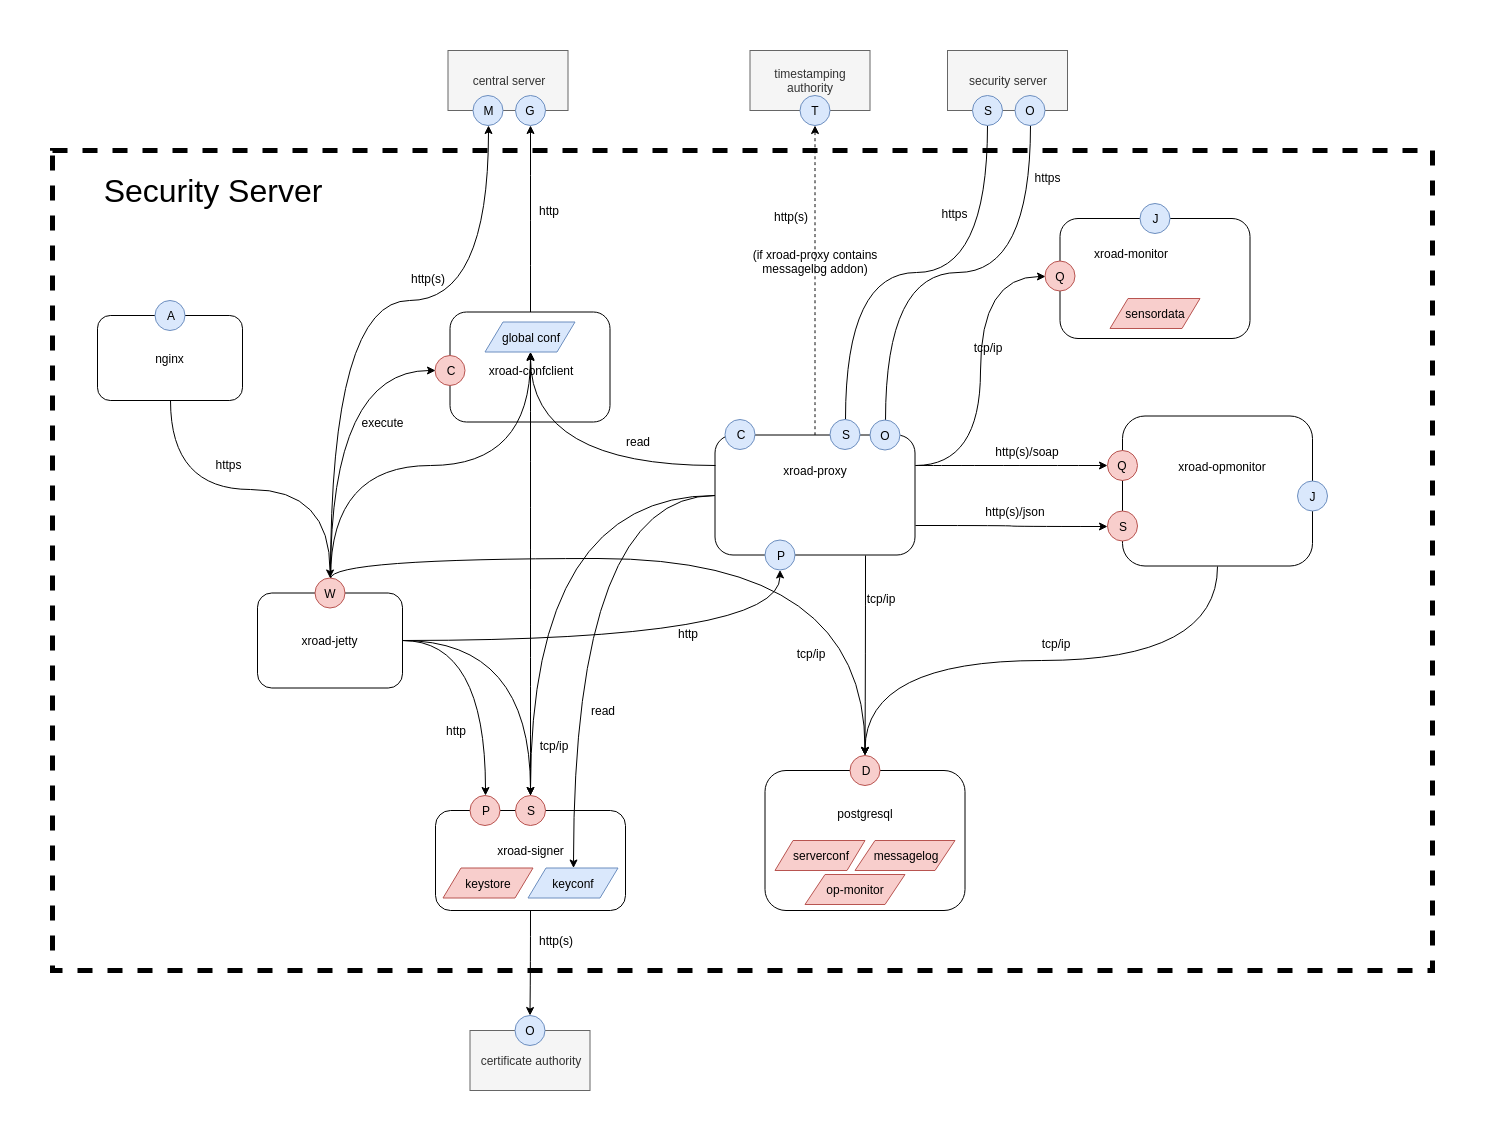
\includegraphics[scale=0.2]{Pictures/arc-ss_security_server_process_diagram.png}
    \caption{Diagrama de Proceso del componente \textbf{servidor de seguridad}}
    \label{fig:SSDP}
\end{figure}
\begin{figure}[h!]
    \centering
    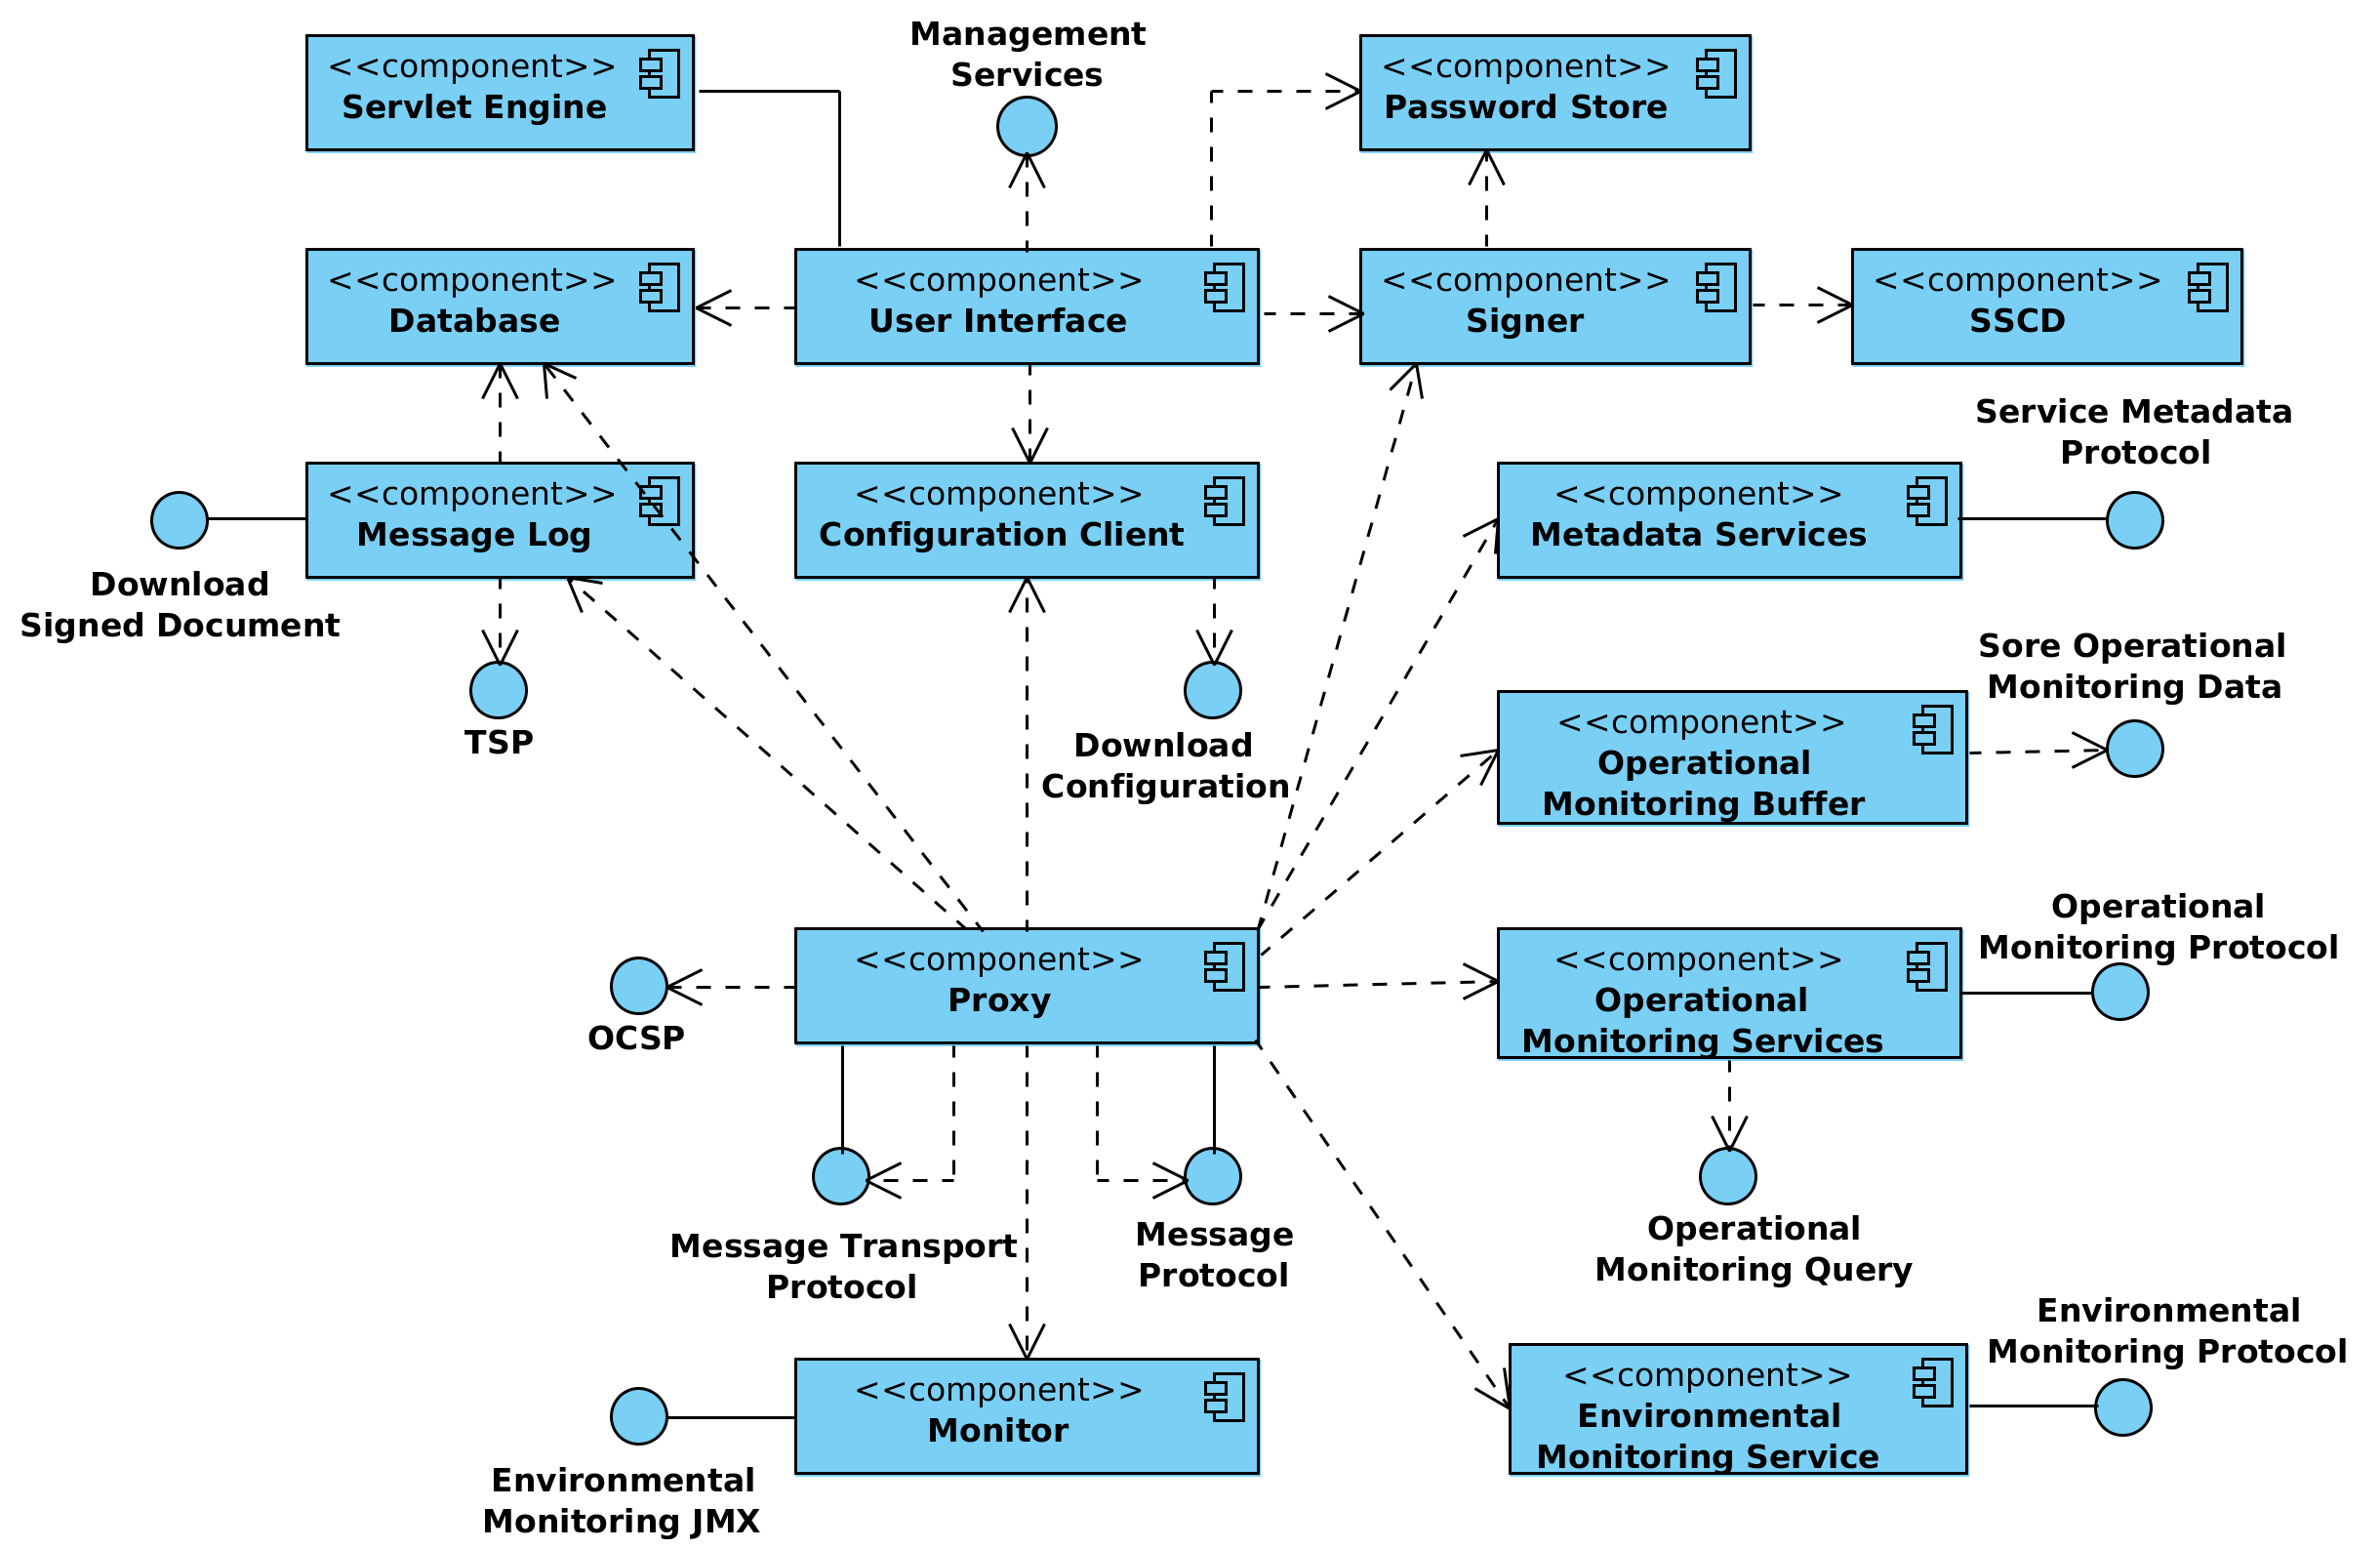
\includegraphics[scale=0.5]{Pictures/arc-ss_security_server_component_diagram.png}
    \caption{Diagrama de componentes del \textbf{servidor de seguridad}}
    \label{fig:SSDC}
\end{figure}

\begin{figure}
    \centering
    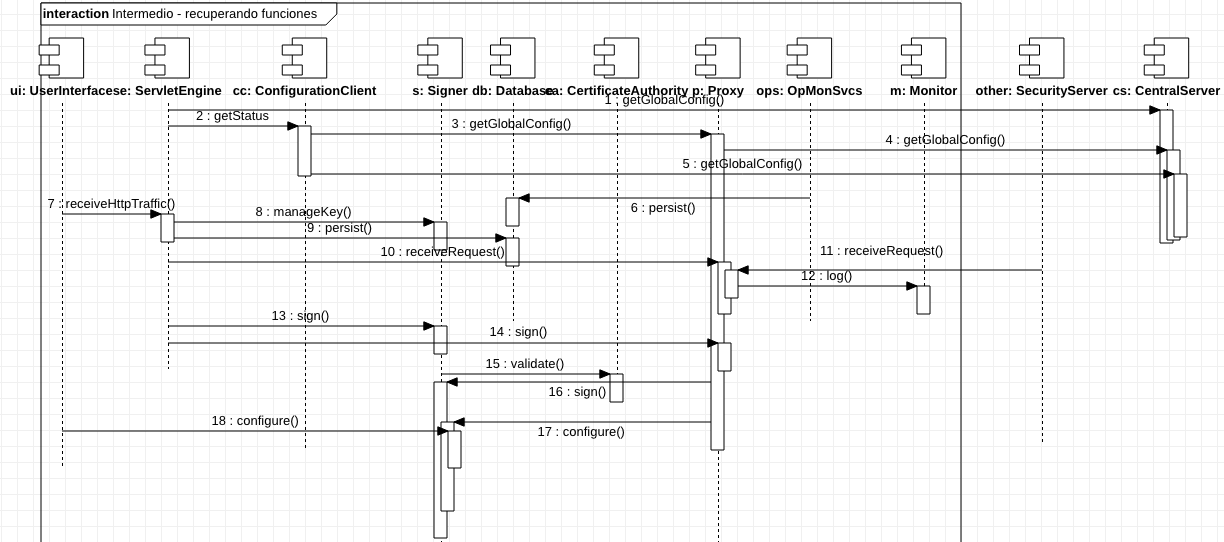
\includegraphics[width=\textwidth]{Pictures/xroad.png}
    \caption{Diagrama de secuencia del Caso hipotético y simplificado del proceso (Pregunta 2)}
    \label{fig:xroad}
\end{figure}